% This template was originally by R. Jacob Vogelstein
% Updated on March 1, 2010 by Noah J. Cowan
% Updated on May 18, 2014 by Brian Weitzner at https://github.com/weitzner/jhu-thesis-template
% Updated on January 29, 2016 by John Muschelli at https://github.com/muschellij2/PhD_Thesis
% Updated on April 13, 2016 by Leonardo Collado Torres and available at https://github.com/lcolladotor/jhu-thesis-template. View (read-only) at Overleaf here https://www.overleaf.com/read/tqdzgmrxgbtg
% Updated on July 17, 2020 by Ben Ackerman and available at https://github.com/benjamin-ackerman/jhu-thesis-template


%% It's your responsability to make sure that your thesis complies with
%% JHU's formatting rules available at https://www.library.jhu.edu/library-services/electronic-theses-dissertations/formatting-requirements/

\documentclass[12pt]{report}

%% This was the setup recommended at https://github.com/weitzner/jhu-thesis-template
% \documentclass[12pt,oneside,final]{thesis}

\pdfminorversion=4\relax
\pdfobjcompresslevel=0\relax
%% Followed the information from https://www.overleaf.com/latex/examples/creating-pdf-slash-a-and-pdf-slash-x-files/bbbycnbyqhnm#.Vw6_XBMrLm1 to create a PDF/A file in Overleaf
\usepackage[a-1b]{pdfx} % Need this to create a PDF/A file
\usepackage{pdfpages}
\pagestyle{myheadings}
%\topmargin=0.25in
\topmargin=0.05in
\textheight=8.15in
\textwidth=5.6in
\oddsidemargin=0.7in
\raggedbottom
\newdimen \jot \jot=5mm
\brokenpenalty=10000


%\usepackage[utf8]{inputenc} % Seems to cause a conflict with fontenc and lmodern
%\DeclareUnicodeCharacter{00A0}{ }
\usepackage[T1]{fontenc}
\usepackage{lmodern} % load a font with all the characters
%\usepackage{hyperref}
\usepackage{tocbibind} % need this to contents adding for TOC
\usepackage{setspace}
\setstretch{1.05}
\usepackage{RJournal_nogeom} % Changes the colors of links among other things
%\usepackage[all]{hypcap}
\usepackage[hypcap=true]{caption}
\hypersetup{linktocpage}
\usepackage{amsmath,amssymb,array}
\usepackage{booktabs}
\usepackage{subfig}

%% load any required packages here
\usepackage{graphicx}
\usepackage{float}
\usepackage{tikz}
\usepackage{graphics}
\usetikzlibrary{positioning}
\usetikzlibrary{shapes,arrows}
\usepackage{dcolumn}
% A math shortcut frequently used by John Muschelli
\newcommand{\bbeta}{\mbox{\boldmath $\beta$}}

%%%%%%%%%%%%%%%%%%%%%%%%%%%%%%%%%%%%%%%%%%%%%%%%%%%%%%%%%%%%%%%%
% DOI from Segmentation
% Don't use - needs hyperref
%%%%%%%%%%%%%%%%%%%%%%%%%%%%%%%%%%%%%%%%%%%%%%%%%%%%%%%%%%%%%%%%
%\makeatletter
%\providecommand{\doi}[1]{%
%  \begingroup
%    \let\bibinfo\@secondoftwo
%    \urlstyle{rm}%
%    \href{http://dx.doi.org/#1}{%
%      doi:\discretionary{}{}{}%
%      \nolinkurl{#1}%
%    }%
%  \endgroup
%}
%\makeatother

%%%%%%%%%%%%%%%%%%%%%%%%%%%%%%%%%%%%%%%%%%%%%%%%%%%%%%%%%%%%%%%%
% StartKNITR STUFF -- added by John Muschelli
%%%%%%%%%%%%%%%%%%%%%%%%%%%%%%%%%%%%%%%%%%%%%%%%%%%%%%%%%%%%%%%%
\usepackage{color}
%% maxwidth is the original width if it is less than linewidth
%% otherwise use linewidth (to make sure the graphics do not exceed the margin)
\makeatletter
\def\maxwidth{ %
  \ifdim\Gin@nat@width>\linewidth
    \linewidth
  \else
    \Gin@nat@width
  \fi
}
\makeatother

\definecolor{fgcolor}{rgb}{0.345, 0.345, 0.345}
\newcommand{\hlnum}[1]{\textcolor[rgb]{0.686,0.059,0.569}{#1}}%
\newcommand{\hlstr}[1]{\textcolor[rgb]{0.192,0.494,0.8}{#1}}%
\newcommand{\hlcom}[1]{\textcolor[rgb]{0.678,0.584,0.686}{\textit{#1}}}%
\newcommand{\hlopt}[1]{\textcolor[rgb]{0,0,0}{#1}}%
\newcommand{\hlstd}[1]{\textcolor[rgb]{0.345,0.345,0.345}{#1}}%
\newcommand{\hlkwa}[1]{\textcolor[rgb]{0.161,0.373,0.58}{\textbf{#1}}}%
\newcommand{\hlkwb}[1]{\textcolor[rgb]{0.69,0.353,0.396}{#1}}%l
\newcommand{\hlkwc}[1]{\textcolor[rgb]{0.333,0.667,0.333}{#1}}%
\newcommand{\hlkwd}[1]{\textcolor[rgb]{0.737,0.353,0.396}{\textbf{#1}}}%

\usepackage{framed}
\makeatletter
\newenvironment{kframe}{%
 \def\at@end@of@kframe{}%
 \ifinner\ifhmode%
  \def\at@end@of@kframe{\end{minipage}}%
  \begin{minipage}{\columnwidth}%
 \fi\fi%
 \def\FrameCommand##1{\hskip\@totalleftmargin \hskip-\fboxsep
 \colorbox{shadecolor}{##1}\hskip-\fboxsep
     % There is no \\@totalrightmargin, so:
     \hskip-\linewidth \hskip-\@totalleftmargin \hskip\columnwidth}%
 \MakeFramed {\advance\hsize-\width
   \@totalleftmargin\z@ \linewidth\hsize
   \@setminipage}}%
 {\par\unskip\endMakeFramed%
 \at@end@of@kframe}
\makeatother

\definecolor{shadecolor}{rgb}{.97, .97, .97}
\definecolor{messagecolor}{rgb}{0, 0, 0}
\definecolor{warningcolor}{rgb}{1, 0, 1}
\definecolor{errorcolor}{rgb}{1, 0, 0}
\newenvironment{knitrout}{}{} % an empty environment to be redefined in TeX
\makeatletter
\newcommand\gobblepars{%
    \@ifnextchar\par%
        {\expandafter\gobblepars\@gobble}%
        {}}
\makeatother
%%%%%%%%%%%%%%%%%%%%%%%%%%%%%%%%%%%%%%%%%%%%%%%%%%%%%%%%%%%%%%%%
% End KNITR STUFF
%%%%%%%%%%%%%%%%%%%%%%%%%%%%%%%%%%%%%%%%%%%%%%%%%%%%%%%%%%%%%%%%


\usepackage[
style = authoryear,
sorting = none,
dashed = false,
maxbibnames = 99,
backend = bibtex,
natbib = true
]{biblatex}

% If you want to exclude some portions from the bibliography
\AtEveryBibitem{
\clearfield{note}
\clearfield{month}
}


\usepackage{enumerate}

%\tolerance=10000

%\makeglossary % enable the glossary
\graphicspath{{rnw_chapter/figure/}{rnw_chapter/}} % change it accordingly!


\setcounter{tocdepth}{4}
\setcounter{secnumdepth}{4}
\begin{document}

\newcommand{\bm}[1]{ \mbox{\boldmath $ #1 $} }
\newcommand{\bin}[2]{\left(\begin{array}{@{}c@{}} #1 \\ #2
             \end{array}\right) }
\renewcommand{\contentsname}{Table of Contents}
\baselineskip=24pt

% Create cover page of dissertation !
\pagenumbering{roman}
\thispagestyle{empty}
\begin{center}
\vspace*{.25in}
{\bf\LARGE{ JHU THESIS TEMPLATE TITLE }}\\
\vspace*{.75in}
{\bf by} \\*[18pt]
\vspace*{.2in}
{\bf Yunfan Fan} \\
\vspace*{1in}
{\bf A dissertation submitted to Johns Hopkins University\\
in conformity with the requirements for the degree of\\
Doctor of Philosophy }\\
\vspace*{.75in}
{\bf Baltimore, Maryland} \\
{\bf August, 2022} \\
\vspace*{.5in}
\begin{small}
{\bf \copyright{ }2022 by Yunfan Fan} \\
{\bf All rights reserved}
\end{small}
\end{center}
\newpage

% Add acknowledgements
\pagestyle{plain}
\pagenumbering{roman}
\setcounter{page}{2}
\chapter*{Abstract}
\label{chap:abstract}
\addcontentsline{toc}{chapter}{Abstract}
\markboth{Abstract}{Abstract}

While next generation sequencing (NGS) has enabled massively parallel DNA sequencing for lower and lower cost, the development of third generation nanopore sequencing offers several key advantages over older sequencing methods. Nanopore sequencers are pocket-sized, making them orders of magnitude cheaper than the next most affordable alternative and the ideal option for wide deployment. They are capable of providing data in real-time, saving valuable hours before data analysis can begin. Additionally, they are able to sequence reads several thousand basepairs long, as opposed to the hundreds of basepairs NGS platforms are capable of, and they embed base modification data without the need for specific treatment beforehand. Given these advantages, in this thesis I examine the application of nanopore sequencing to the study of human pathogens.

First, we use nanopore sequencing to characterize anti-microbial resistance (AMR) in forty clinical isolates. We analyzed real-time data to quickly identify AMR genes, assembled genomes to identify chromosomal mutations, and used short-read sequencing data to correct the errors in the assemblies. With sequencing data, we found that time to effective antibiotic therapy could be shortened by as much as 20 hours compared to standard antimicrobial susceptibility testing (AST).

Second, we leverage the long reads of nanopore sequencing to assemble the genome of a pathogenic yeast, /textit{Candida nivariensis}. Previous efforts to assemble this yeast genome relied solely on NGS data, resulting in a highly fragmented genome. Using nanopore data, we achieve a much higher contiguity, capture previously missing portions of the genome. Furthermore, we demonstrate that our more contiguous genome can be used to better study long and repetative genes, such as those involved in pathogenticity to humans.

Third, we use the base modification information embedded in nanopore sequencing data to call methylation in metagenomic assemblies. These calls enable the binning of metagenomic contigs according to methylation signature without the need to collect additional data. We demonstrate the efficacy of this method on a synthetic community sample, a simple two-bacteria system, and a clinical sample with matched proximity ligation binning data.

These applications of nanopore sequencing demonstrate its potential and its utility for all fronts of pathogen genomics research.

\chapter*{Thesis Committee}

\section*{}

\begin{singlespace}


\indent Dr. Winston Timp (Advisor, Reader)\\
\indent \indent Associate Professor \\
\indent \indent Department of Biomedical Engineering \\
\indent \indent Department of Molecular Biology and Genetics \\
\indent \indent Johns Hopkins University School of Medicine \\



\smallskip

\noindent Dr. Patricia Simner (Reader) \\
\indent \indent Associate Professor \\
\indent \indent Department of Pathology \\
\indent \indent Johns Hopkins University School of Medicine \\


\smallskip

\noindent Dr. Steven Salzberg \\
\indent \indent Bloomberg Distinguished Professor \\
\indent \indent Department of Computer Science \\
\indent \indent Johns Hopkins University Whiting School of Engineering \\
\indent \indent Department of Biomedical Engineering \\
\indent \indent Johns Hopkins University School of Medicine \\
\indent \indent Department of Biostatistics \\
\indent \indent Johns Hopkins Bloomberg School of Public Health \\



\end{singlespace}

\chapter*{Acknowledgments}

I have tremendous gratitude \\
to those people, \\
numerous and innumerable, \\
who have contributed, \\
directly or in subtler ways, \\
to this work.

Some of them are listed here. \\

\textbf{To my advisor, Winston:} I remember writing to you as a sophomore in college many years ago, asking to do research in your brand new lab, which at the time was but a few months old. Back then, I had no idea what it was to do research, and I had no relevant skills or credentials to offer, only my time and my interest to learn. Over these years I have indeed learned a lot, and I will always be grateful to you for building the place where I was able to grow.

\textbf{To my thesis committee, Trish and Steven:} Thank you for your exceptionally kind guidance, support, and feedback. I always left committee meetings with you feeling more confident in myself, and more optimistic about my progress.

\textbf{To the @yfan arc of the \texttt{\#}core channel - @isac, @brochael, @shao, @gilfunk, @narley, @broham, @gmoney, @Brittany, @sherbear, @Sam Sholes, @Paul Hook, @amymeltzer39, @alice, @Luke Morina, @Courtney Johnson, and @Jess:} Thank you for those times when you patiently watched over me as I learned new lab techniques, answered my dumb questions, and generally rescued me from predicaments of my own making. It is my fondest hope that at some point during our time together, I was able to reciprocate by being even mildly helpful. Thank you most of all for commiserating with me as we struggled together through the singular challenges of research, and celebrating the equally singular triumphs.

\textbf{To the crew that moved me into 703 (and Charles, and Charlotte, and Sven, and Manolo):} Thanks for being there, and thanks for hanging out. Let's go climbing and get a beer the next time we're all around. It's been a while.

\textbf{To mom and dad, and family further away:} It was your labor that first cultivated my growth. Accomplishments in my name are as much yours as they are mine. I flourish for you.


%\cleardoublepage
%\newpage
\pagestyle{plain}
\baselineskip=24pt
\tableofcontents
% for the three lines below, change the page numbers if needed!
%\addtocontents{toc}{\contentsline{chapter}{Table of Contents}{iii}}
%\addtocontents{toc}{\protect\contentsline{chapter}{\protect\numberline{}Table of Contents}{iii}}
%\addtocontents{toc}{\protect\contentsline{chapter}{\protect\numberline{}List of Tables}{iv}}
%\addtocontents{toc}{\protect\contentsline{chapter}{\protect\numberline{}List of Figures}{v}}
\listoftables
\listoffigures

\cleardoublepage % Needed because our intro chapter doesn't really have anything
\pagenumbering{arabic}


% add your chapters, best way is to have separate TeX files for each chapter
%\include{chapter0}
%\include{chapter1}

%% The above was the recommended setup by https://github.com/weitzner/jhu-thesis-template but it's no longer needed
%% after Muschelli's changes which stores different chapters in their
%% respective directories. You will still need to add your chapters as
%% TeX files or Rnw files (see rnw_chapter as an example) and please
%% remember to update the makefile accordingly.

\begin{refsection}[intro_chapter/intro_chapter.bib]
\chapter{Introduction}
\label{chap:intro}

\section{Sequencing Technology}
\label{sec:seq}
Since Sanger developed a chain-terminating procedure for DNA sequencing over forty years ago \citep{Sanger1977-lo}, sequencing capabilities have grown, at first steadily, then astronomically \citep{Schatz2013-vw}. The advent of sequencing-by-synthesis ushered in ‘next-generation’ sequencing (NGS) methods, whereby DNA sequencing became ‘massively parallel’ in nature and vastly accessible to researchers in all fields of biology and medicine. These NGS methods typically involve immobilizing millions of DNA fragments, amplifying them, and then observing the activity of DNA polymerase as it synthesizes the complement strands to the amplified fragments. Commonly, this observation is done through imaging fluorescently labeled nucleotides one base addition, or cycle, at a time \citep{Shendure2017-oy}.

The highly democratized nature of NGS has enabled researchers in clinical microbiology to use it for a variety of important applications. These range from cataloging and surveilling genetic determinants of antimicrobial resistance (AMR) \citep{Crofts2017-ni, Canica2019-ho, Toth2020-ov, Thanner2016-wy, Hendriksen2019-qi}, to monitoring outbreaks of infectious diseases \citep{Dipaola2020-bw, Lu2020-ti}, to analyzing entire human microbiomes with metagenomic sequencing \citep{Chiu2019-cg}. Based on the advances brought about by NGS, some have even called for establishing a ‘digital immune system’ whereby sequencing-based microbial surveillance would detect threats of outbreak, which then could be contained before they become too difficult to control \citep{Schatz2012-ow}.

While NGS technology has unlocked enormous advances in clinical microbiology, it is limited by the fragment lengths it can handle and its reliance on amplification. Typical NGS methods are unreliable at sequencing individual DNA fragments multiple thousands of base pairs long \citep{Heather2016-wb}, and can only read stretches of a few hundred nucleotides at a time. These short read lengths make the sequencing data difficult to work with for many downstream applications, including genome assembly and analysis of repetitive genomic loci. Meanwhile, the amplification process obliterates any base modification information, such as methylation, potentially present on the native DNA fragment.

The rise of third generation, single-molecule sequencing just in the past decade has begun to address these shortcomings. These methods, also known as ‘long-read’ sequencing, interrogate individual DNA molecules without the need for amplification, and can read stretches of thousands of nucleotides at a time \citep{Jain2018-qp}. Nanopore sequencing in particular does this by measuring the minute fluctuations in ionic current as a single stranded DNA molecule passes through a transmembrane protein pore. Because no amplification or other chemical treatments are required prior to sequencing, base modification information remains intact and can be read simultaneously with the nucleotide sequence \citep{Simpson2017-wb, mcintyre2019single}. Also unlike NGS methods, the current single molecule sequencing procedures are not dependent on imaging single bases from all the reads at once in a synchronized fashion. Data is collected from all pores independently, which enables data streaming to analysis pipelines even as more data are still being collected. To further the role of sequencing for infectious disease applications, I leverage the new capabilities of nanopore sequencing for AMR detection, genome assembly of eukaryotic pathogens, and metagenomics.

\section{Antimicrobial resistance}
\label{sec:amr}
Since Alexander Fleming first observed the ‘bacteriolytic’ properties of a mysterious ‘mould broth filtrate’ which he termed ‘penicillin’ \citep{Fleming1929-cb}, antibiotics have been an unprecedented and miraculous silver bullet against previously deadly bacteria. Usually produced and isolated from fungi \citep{Martinez2008-cf}, antibiotics are small molecules capable of killing bacteria or inhibiting their growth without damaging eukaryotic cells or tissues in the vicinity. Not only are antibiotics used to cure infectious diseases, but they have enabled more and more complex medical interventions such as surgery and chemotherapy by drastically reducing the risk and ramification of bacterial infections \citep{Crofts2017-ni}. Outside of medicine, antimicrobials have also been used extensively in animal agriculture to control disease \citep{Aarestrup2015-zu}, as populations of food animals are scaled to accommodate global diets that continue to demand more animal protein \citep{Van_Boeckel2019-zl}. Consequently, antibiotics are one of the most commonly prescribed classes of drugs in recent decades, and their use is only becoming more widespread \citep{Van_Boeckel2014-io}.

However, for as long as fungi have produced antimicrobials, bacteria have evolved resistances to them \citep{DCosta2011-yn}. As human usage of antibiotics has occurred ubiquitously and without restraint, selection pressures have caused a rapid proliferation of antibiotic resistant strains of bacteria. Even synthetic antibiotics such as quinolones sustained only three decades of widespread usage before resistances began to develop, intensify, and spread \citep{Laxminarayan2013-dk, Ruiz2012-cx}. Multidrug-resistant strains of bacteria have also emerged and become prominent, deepening the international crisis of AMR \citep{Tamma2014-dh}.

In the clinic, the prevalence of AMR makes it difficult to immediately prescribe the most effective interventions for patients colonized with commonly drug resistant bacteria. Not only does this cost potentially crucial time from patient treatment, but it could cause antibiotic waste and contribute to selection pressures causing drug resistances to develop in the first place. In Chapter 2, I explore the use of third generation sequencing in the clinic to rapidly detect drug resistances in order to shorten the time to effective antibiotic therapy and enable antibiotic stewardship.

\section{Genome Assembly}
\label{sec:asm}
High quality, complete genomes are crucial not only for population and comparative genomics, but they also commonly underpin gene expression studies, epigenetics assays, and molecular diagnostics \citep{Rhie2021-xb}. Because highly parallel sequencing technologies cannot record whole genomes on a single read, genomes must be reconstructed out of millions or billions of reads. This process has been likened to a large jigsaw puzzle, where reads must be overlapped, oriented and fit together in order to build the larger picture of the genome \citep{Sohn2018-lf}. Contiguous sequences constructed by overlapping reads in this fashion are known as ‘contigs,’ which typically represent large sections of chromosomes.

Repetitive and low complexity regions of the genome have been difficult to resolve using NGS technologies. The short reads often cannot span these regions, making it difficult to unambiguously determine how long they are, and how many repeats each region contains \citep{Paszkiewicz2010-yf}. Contigs are typically terminated at these ambiguous regions, resulting in highly fragmented assemblies containing thousands of contigs. Long read data capable of spanning repetitive regions are able to resolve the ambiguities they cause, resulting in much more contiguous genome assemblies with longer and fewer contigs. Genome assemblies constructed from only long read data are more prone to single-base errors due to the lower accuracy of the long reads, but NGS data gathered on the same sample can be used to correct most small errors \citep{Goodwin2015-qs}. Using both long-read and NGS data leverages the benefits and addresses the weaknesses of both sequencing technologies.

Only with contiguous, reference-quality genome assemblies can the roles of repeat structures and long, repetitive genes be analyzed. In pathogenic fungi, some adhesion proteins tend to be encoded in long genes with tandem repeats embedded within. These proteins are of particular interest as they are thought to be involved in enabling pathogenicity \citep{Timmermans2018-ci}. In Chapter 3, I use both NGS and long-read data to assemble the genome of \textit{Candida nivariensis}, a pathogenic yeast, and use the assembled genome to explore the long, repetitive genes encoding adhesions in this species.

\section{Metagenomics}
\label{sec:asm}
Microbes are ubiquitous, and structured microbial communities, or microbiomes, can be found associating with a variety of hosts and environmental niches \citep{Quince2017-ay}. Increasingly, the human associated microbiomes are found to play an important role in human health \citep{Fan2021-hh}. Studying complex communities using traditional microbial methods based on culturing bacteria has been difficult, as not all microbes can be cultured, and the culturing process itself would be likely to alter the composition of the community \citep{Quince2017-ay}.

Community members can be identified and quantified using 16S rRNA sequencing, whereby the 16S genes of all microbial genomes in the community are simultaneously amplified, and then sequenced. By comparing only these 16S sequences to each other and to reference databases, operational taxonomic units (OTUs) making up the community can be determined, and taxonomy can be assigned \citep{Johnson2019-wk}. While 16S-based methods are effective for studying the organism composition of microbiomes, it cannot directly shed any light on the functional capabilities of the microbes.

By contrast, metagenomics sequencing captures the full genetic complement of the community, including any genes, plasmids, or phages which may be present in the cells and their environs. While more sequences are captured with metagenomics, analyzing this data becomes more difficult computationally \citep{Breitwieser2019-zp}. One common approach to analysis involves assembling the metagenome in order to determine identity and functions of the microbes in the community \citep{Lapidus2021-dj}. Metagenome assembly is functionally similar to genome assembly of a single organism, where reads are overlapped in order to construct contigs. However, because metagenomic contigs can originate from an undetermined number of organisms, grouping, or ‘binning,’ these contigs according to the species of origin is a crucial yet challenging step in metagenomic analysis \citep{Yue2020-cm}.

Binning metagenomic contigs into metagenome assembled genomes (MAGs), using NGS data has typically been done using a combination of the contigs’ kmer-spectra, and differential coverage \citep{Ghurye2016-mb}. While these methods work well for bacterial chromosomes, they are less effective for binning mobile genetic elements (MGEs), especially if these MGEs are capable of replicating independently of the host chromosome, as most plasmids are. As with genome assembly of a single organism, the use of NGS data in metagenomic assembly limits the lengths of the contigs themselves, potentially resulting in unresolvable repeats and truncated gene sequences.

By applying long-read sequencing to metagenomic analysis, it is possible to assemble much longer contigs from microbiome samples. Furthermore, because native base modification information is preserved, it can be a powerful basis for binning, as modifications are preserved on MGEs and are not affected by chromosome-independent replication. In Chapter 4, I use methylation calls derived from nanopore sequencing for metagenomic binning, and assess its effectiveness.

\cleardoublepage
\printbibliography[title={References}]
\end{refsection}


\begin{refsection}[rnw_chapter/rnw_chapter.bib]
\chapter{Genome assembly of Candida nivariensis}
\label{chap:rnw}





This document was generated on Mon May  2 14:39:59 2022.

As shown in Figure \ref{fig:myfig} and in Table \ref{tab:rtab1} we can see that bla bla \citep{B}.


\begin{figure}[!ht]
\centering
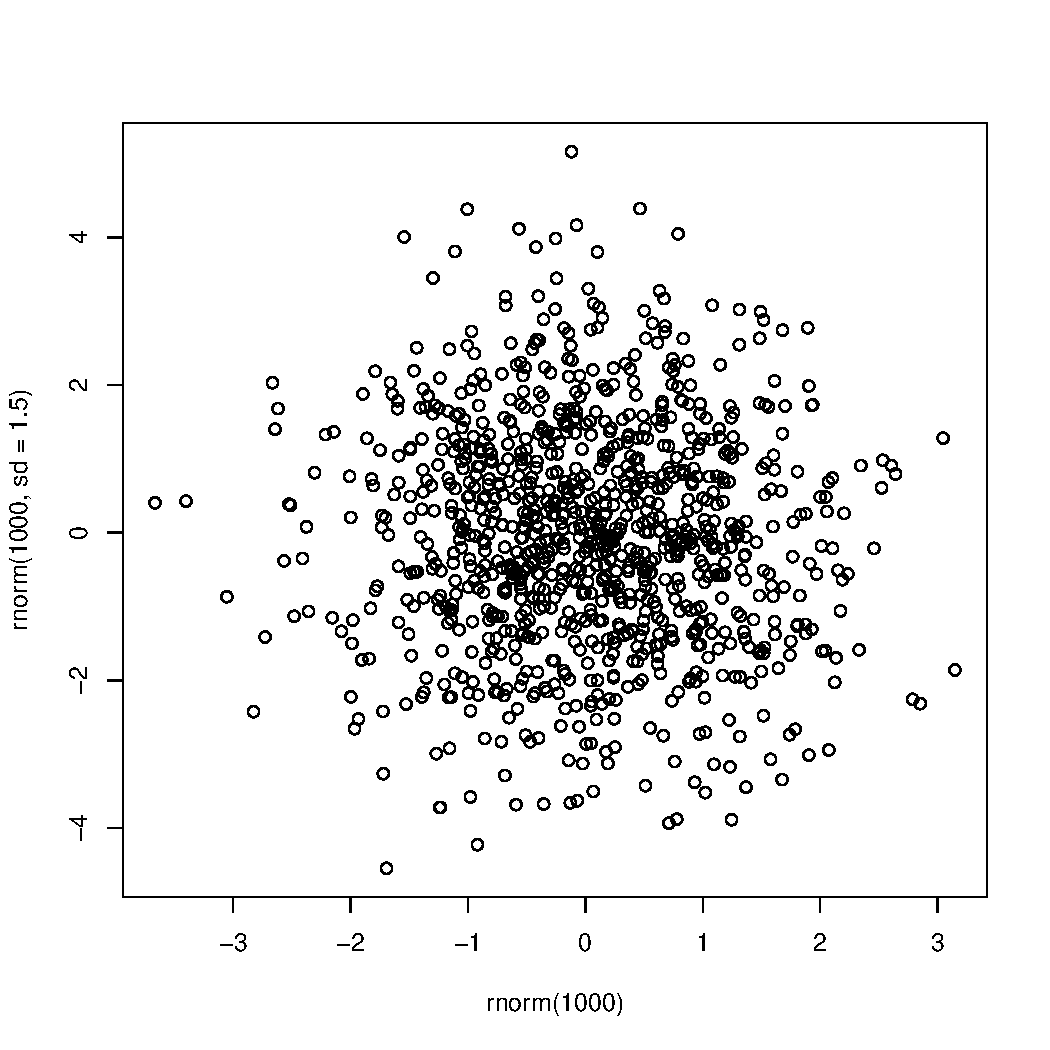
\includegraphics[width = 1\linewidth,keepaspectratio]{figure/myfig.pdf}
\caption[Some random figure]{{\bf Some random figure.} {\bf (a)} blah first point {\bf (b)} blah second point {\bf (c)} blaih thrid panel  }
\label{fig:myfig}
\end{figure}




% latex table generated in R 3.6.3 by xtable 1.8-4 package
% Mon May  2 14:39:59 2022
\begin{table}[ht]
\centering
\begin{tabular}{rr}
  \hline
A & B \\ 
  \hline
  1 & -1.01 \\ 
    2 & -1.46 \\ 
    3 & 0.13 \\ 
    4 & -0.17 \\ 
    5 & 0.40 \\ 
    6 & -0.00 \\ 
    7 & -1.34 \\ 
    8 & 0.31 \\ 
    9 & 0.29 \\ 
   10 & 0.49 \\ 
   \hline
\end{tabular}
\caption{\bf{ Table title } Table description} 
\label{tab:rtab1}
\end{table}


\cleardoublepage
\printbibliography[title={References}]
\end{refsection}

\begin{refsection}[conclusion_chapter/conclusion_chapter.bib]
\chapter{Discussion and Conclusion}
\label{chap:conclusion}

As infectious diseases continue to be of growing interest and concern \citep{Baker2022-eb}, methods to monitor, diagnose, understand, and combat them must continue to evolve and improve. Sequencing technologies have developed at breakneck pace in recent decades \citep{Hu2021-dd, Schatz2013-vw}, and sequencing based investigative methods have been applied to great effect in almost all fields of biology and medicine. I have taken advantage of the unique properties of the most recent generation of sequencing technology for infectious disease applications, using it to identify and surveille AMR genes, assemble eukaryotic pathogen genomes, and link plasmids to hosts in complex microbial communities.

While nanopore sequencing can detect specific AMR genes quickly and agnostically \citep{Tamma2019-jg}, it can still be difficult to infer phenotypic resistance \citep{Yee2021-td}. Genomic data is able to provide information on an organism’s potential behavior, but observations of actual activity and function require transcriptomic or proteomic data. In situ functional studies of resistance mechanisms with metatranscriptomics could help to address these issues. As understanding of resistance mechanisms continues to grow, predictions of phenotypic resistance will become increasingly accurate and clinically actionable.

Use of long read sequencing for genome assembly has unlocked continuously larger genomes \citep{Neale2014-di}, and accompanying software has made high quality genome assembly more accessible than ever before \citep{Fan2021-cq}. As more and more eukaryotic pathogen genomes are sequenced, collated, and curated \citep{Aurrecoechea2017-tl}, they will become crucial to the development of sequencing-based diagnostics of infectious diseases \citep{Lu2018-wr}, in addition to being useful for furthering basic science research on these organisms.

Long-read data for metagenomic assembly not only produces longer contigs, but is able to preserve base modification data, which can be used for binning applications. Not only can contigs be grouped on the bases of base modifications, but reads can as well. Although this has not been shown using a single nanopore run, its possibility has been demonstrated using PacBio data \citep{Beaulaurier2018-mu}. Developing this capability in nanopore sequencing would enable multi-host plasmid assignments which are currently unfeasible.

\cleardoublepage
\printbibliography[title={References}]
\end{refsection}


% CV PDF file downloaded from the moderncv template available at Overleaf
% https://www.overleaf.com/latex/templates/modern-cv-and-cover-letter-2015-version/sttkgjcysttn#.Vw6PFRMrL65
\addcontentsline{toc}{chapter}{Curriculum Vitae} % CV must be in table of contents
\includepdf[pages={-}, pagecommand={}]{moderncv-2015.pdf} %continue page numbering through CV


\end{document}
